
\chapter{全局路径规划导航方法}
为实现移动机器人既能根据自然语言指令中的目标进行导航,又能完成导航至目标半米内的任务,本文提出了一种语言视觉激光多模态融合的机器人导航(Language Vision Lidar Navigation, LVL-Nav)方法。为了能够完成上述任务,我们提出的LVL-Nav将导航任务拆分为已知环境中下的全局路径规划导航和未知环境下的局部路径规划两个部分。本章将详细介绍LVL-Nav方法中的全局路径规划导航方法。主要有目标物体导航任务定义,然后描述了所提出的全局路径规划导航方法的框架设计,最后分别描述了框架中的指令语义提取模块、多模态融合网络模块、方位优化算法和导航点规划算法四个部分。其中指令语义提取模块将非结构化的语言指令通过大语言模型映射到具体的目标空间和方位空间,前者作为多模态融合网络模块中的目标特征与图像编码器和深度图编码器所提取环境的图像特征、深度特征拼接得到的环境特征进行跨模态融合,帮助智能体理解多种模态之间的关系;后者则通过方位优化算法辅助筛选掉冗余的导航点,最后再通过导航点规划在最大化目标与导航点的匹配程度的同时最大化导航成功率。

\section{导航任务定义}
多模态融合的目标物体导航任务要求代理从室内环境中的随机起始位置根据自然语言指令导航到用户依次指定的物体类别,如打印机、餐桌、储物柜等,并且代理被允许使用以第一视角的视觉观察(通常为RGB图像)和激光雷达,其问题可以定义如下:给定自然语言指令$I$和智能体在环境中的初始位姿$S$,通过解析指令要求,在建好的栅格地图中的导航点集中依次推理选择与指令目标序列$\left\{ {{l_i}} \right\}$相匹配的导航点序列$\left\{ {{v_i}} \right\}$,并最终在目标位置的半米内停下以完成导航任务。

一次完整的目标物体导航过程如图\ref{simularity_world}所示,代理在t=0的初始时刻被初始化在房间右上角餐桌附近的$S$点,同时能获得单目相机和激光雷达第一视角的RGB图像和点云数据,以及一条导航指令“Go all the way to the refrigerator, then turn around to the sofa, straight forward past the bed, and stop at the edge of the chair.”。然后代理通过全局路径规划生成任务执行序列,随后在构建的拓扑路径网络中进行节点间的移动,需要在餐桌附近依次导航到冰箱、沙发、寝室的床和床边的座椅,在经过所有子目标之后在最终目标的位置附近停下。其中,蓝色箭头依次所指的目标是智能体所推理出的所有目标节点。
\begin{figure}[htbp]
    \centering
    \includegraphics[scale=0.05]{Fig/target_nav.png}
    \caption{\label{simularity_world}目标物体导航过程}
\end{figure}



\section{导航框架设计}
目标物体导航是机器人导航中的一个重要子任务和研究方向,其主要目的是通过代理对环境的感知和认知信息依次到达指令给定的目标物体。现有的目标物体导航方法中,
Ke\cite{ke2019tactical}等人提出了一种FAST模型,使用贪婪搜索算法将目标对象描述的编码与动作空间的编码相结合,以导航到下一个目标点。
Hong\cite{hong2020language}等人提出了一种新的语言和视觉实体关系图,通过在语言元素与视觉实体之间传递信息,实现了不同模态之间的高效协同,并将其用于捕捉并模拟文本与视觉之间以及视觉实体之间的相互关系。
Wang\cite{wang2021structured}等人针对代理无法实时捕捉环境布局和进行长期规划这一限制,提出了一种结构化场景记忆(Structured Scene Memory, SSM)导航框架,它可以自适应地捕获和表征环境中的视觉和几何特征以支持当前决策,并模拟迭代算法进行远程推理以实现高效的全局规划,他们的算法在R2R和R4R数据集上的实验结果取得了最优秀的性能。
Pashevich\cite{}等人针对代理无法准确地处理长序列的子任务和理解复杂的人类指令,提出了一种多模态转换器(Episodic Transformer, E.T.),利用合成指令作为中间表示,将理解环境的视觉特征与复杂多样的自然语言指令解耦。
Shah\cite{shah2021ving}等人提出的视觉语言导航方法使机器人能够根据目标图像和环境拓扑图进行导航。
Huang\cite{huang2023visual}等人创新性地提出了一种基于空间映射表示的方法VLMaps,它直接将预训练的视觉语言特征与物理世界的3D重建融合在一起,通过大语言模型可以将自然语言命令转换为一系列可以定位在地图中的开放词汇导航目标,并且允许在多个机器人之间共享以动态生成新的障碍地图。
王湉\cite{王湉2024基于大语言模型的人机交互移动检测机器人导航方法}等人通过场景语义分割和三维重建的方法构建语义地图,再利用语言模型理解并执行指令。

这些目标物体导航方法如图\ref{preview_problem}所示,他们大都强调在环境中提取物体语义、位置、物体关系等丰富的视觉特征表示,并将其与栅格地图中的导航点相关联,以此来告诉代理应该导航到哪个导航点,但这种做法过于关注环境中存在什么物体,缺失了已知环境的拓扑信息,没有利用语义中的方位信息进行导航点的筛选,且视觉语言模型在光线条件变化大的室内的鲁棒性较低,从而导致了导航成功率和导航效率低的问题。
\begin{figure}[htbp]
    \centering
    \includegraphics[scale=0.07]{Fig/pre_problem.png}
    \caption{\label{preview_problem}之前工作存在的问题}
\end{figure}

因此,如何在进行图像观察中的物体语义、位置、物体关系等目标物体视觉表示和栅格地图中所标记导航点的匹配过程中,利用环境中不同导航节点和机器人当前位姿所构成的拓扑信息来辅助代理进行更精确地匹配,优化传统的视觉语言模型以克服其在曝光或欠爆环境下模型性能差的问题,再通过从语言指令中提取的方位信息进行方位优化以筛选掉不在目标方向上的冗余导航点,从而提高指导代理依次导航到目标点的导航成功率和导航效率。

在全局路径规划中我们的导航框架如图\ref{global_framework}所示。$添加流程图及其相应的解释$全局路径规划主要由四个关键模块算法构成。首先,输入的导航指令在经过大语言模型处理之后得到目标序列和动作序列,前者与环境中存在的多个可能的导航点图像一同作为多模态融合网络的输入得到导航点匹配特征,后者在经过方位优化算法后筛选掉冗余的导航点,再基于栅格地图和初始位姿计算获得环境的拓扑图以补足环境拓扑特征,最后通过导航点规划算法综合考虑多种导航策略以获得最终的导航点序列,依次发布导航点以完成导航任务。

我们的方法考虑了之前工作中不足的地方并加以改进。具体来说,视觉图像导航方法的效果在很大程度上取决于多模态融合网络的性能,多模态融合网络通过引入深度信息,优化传统视觉语言模型,提高模型在光线条件变化大的室内的鲁棒性,此外,本文针对室内环境存在多种相同目标的情况,提出了一种方位优化方法,结合指令中提供的方位信息与移动机器人的实时位姿,筛选不符合方位条件的冗余导航点,进一步提高全局路径规划中导航点与目标匹配的正确率,最后通过环构建的环境拓扑图结合上述两个算法结果进行导航点规划算法,最终获得导航点序列以执行全局路径导航。
\begin{figure}[htbp]
    \centering
    \includegraphics[scale=0.09]{Fig/global_framework.png}
    \caption{\label{global_framework}全局路径规划导航框架}
\end{figure}


\section{指令语义提取模块}
房间到房间(Room-to-Room,R2R)是一个用于验证视觉语言导航(VLN)模型的基准数据集\cite{anderson2018vision}。该数据集的环境信息通过拓扑导航网络进行表示,如图\ref{r2r_nav}所示,其中每个顶点代表移动机器人在环境中的可达点,同时该点还会对应一个在该位置获取的360度全景视觉观测,连接于顶点之间的边则代表可达性关系。目标物体导航任务要求智能体根据输入的自然语言指令生成正确的目标点导航序列。举例来说在给出指令“Turn left and exit the room. Keep walking along the hall past the kitchen area. Wait by the doorway to the dining table area.”后,智能体根据对指令的理解从起始点开始执行导航任务,它需要根据推理的结果在导航图的节点间进行移动并最终到达目标位置。
\begin{figure}[htbp]
    \centering
    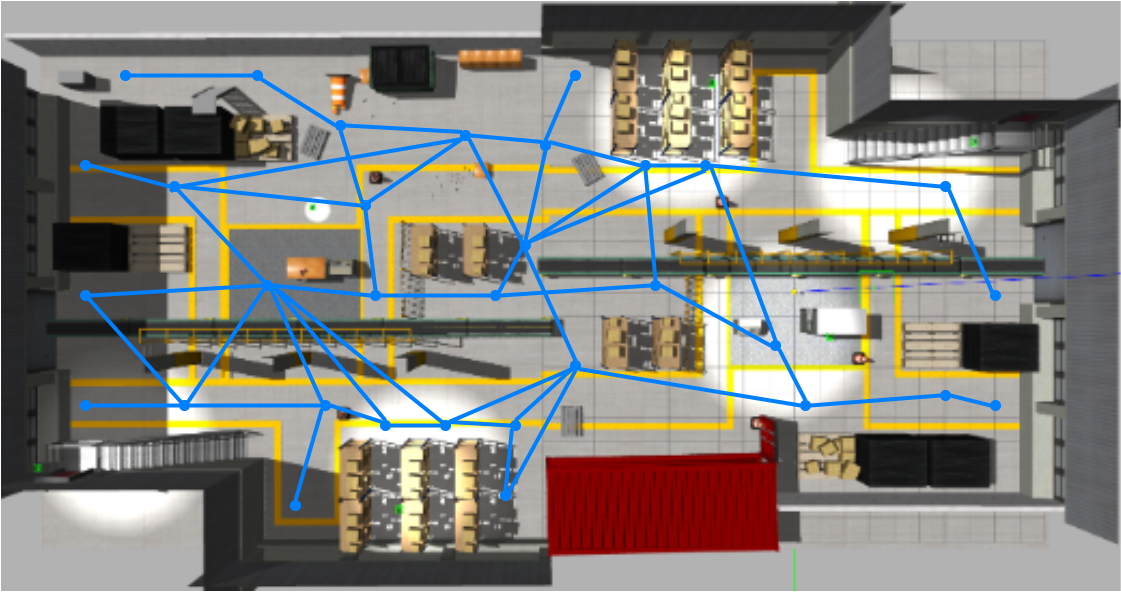
\includegraphics[scale=0.35]{Fig/导航图示例.png}
    \caption{\label{r2r_nav}导航图示例}
\end{figure}

视觉语言导航技术使人类能够使用自然语言与机器人进行交互,使机器人能够基于对环境的感知和对语言指令的理解来执行相应的导航任务。但目前大多数关于视觉语言导航的研究仍然面临诸多挑战,其中最突出的问题之一是这类方法难以适应人类语言的复杂性和多样性,因为许多现有方法往往忽视或无法全面提取指令中所蕴含的例如目标位置和方位描述这类关键信息,这在很大程度上限制了该技术在实际智能制造环境中的广泛应用。通过统计R2R数据集中存在的部分指令的得到单词分布图\ref{instruction_words}。就分布结果表明我们可以通过利用大语言模型来更准确地解析指令中的目标和方位信息,基于提取出的方位信息可以使智能体更有效地过滤掉复杂室内环境中由于方向不同而产生的大量错误目标,从而显著提升导航任务的执行精度和鲁棒性。这一能力对于提高视觉语言导航系统的实际应用价值至关重要。
\begin{figure}[htbp]
    \centering
    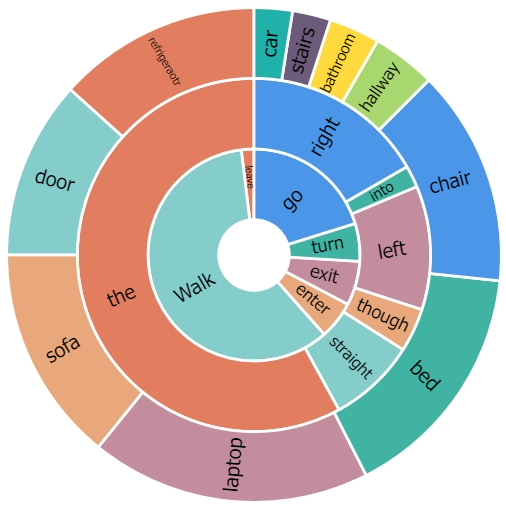
\includegraphics[scale=0.65]{Fig/my_instruction_words.png}
    \caption{\label{instruction_words}R2R指令集中的方位指示分布}
\end{figure}

本文提出并采用了一种专门设计的任务提示模板来解析指令中的目标和方位信息,该模板能够高效且准确地引导语言模型将各种不同形式的导航指令解析并转换为导航任务执行所需的具体目标和方位序列。通过这种方法我们能够为多模态融合网络以及方位优化算法提供更加清晰且具体的任务语义信息,从而提升导航系统的理解能力和执行效率。在实验的过程中我们通过输入任意形式的导航指令,选用了Noun Chunks、GPT3.5、GPT4.0和深度求索(DeepSeek)四种不同的语言模型进行自然语言导航指令解析测试,测试结果如表\ref{deepseekcmp}所示。
\begin{table}
\caption{\label{deepseekcmp}不同的语言模型测试结果}
\centering
\small
\begin{tabular}{cccc}
    \hline
    Noun Chunks & GPT3.5 & GPT4.0 & DeepSeek \tabularnewline 
    \hline 
    0.80 & 0.88 & 0.96 & 0.96 \tabularnewline
    \hline 
\end{tabular}
\end{table}
实验结果表明在我们设计的导航指令提示任务中,Noun Chunks和GPT3.5对复杂句式的处理能力较差,在面对简写、俚语等语言变体导航指令时输出的目标序列和方位序列存在错误、乱序的情况,这样的解析结果会影响系统整体导航的成功率。除此之外,虽然GPT4.0在我们设计的任务中取得了较好的结果,但是移动机器人在接收指令后的很长一段时间都在等待模型响应,其缓慢的响应速度会降低系统整体的导航效率。而DeepSeek则通过垂直领域预训练、知识增强和验证机制的技术路线,在保证它本身能准确地完成特定的语言推理任务的同时还能快速高效地进行响应,因此本文选用DeepSeek\cite{guo2025deepseek}作为核心语言模型。

为了提高语言模型提取结果的准确性,我们通过详细描述任务内容同时提供正确的目标与方位提取示例来引导模型学习合理的输出模式,使其生成的结果尽可能符合预期要求。具体来说在输入一条随意表达的导航指令后,该模型会自动分析并提取句中所包含的目标与方位信息,并将其转换为标准化的数据格式以方便后续导航任务的执行。模型的提取示例结果如图\ref{Extract_orien}所示,在我们的实验测试中该模型对不同风格的导航指令均表现出较高的适应能力和准确性,这进一步证明了该方法在导航任务中的有效性。


\begin{figure}[htbp]
    \centering
    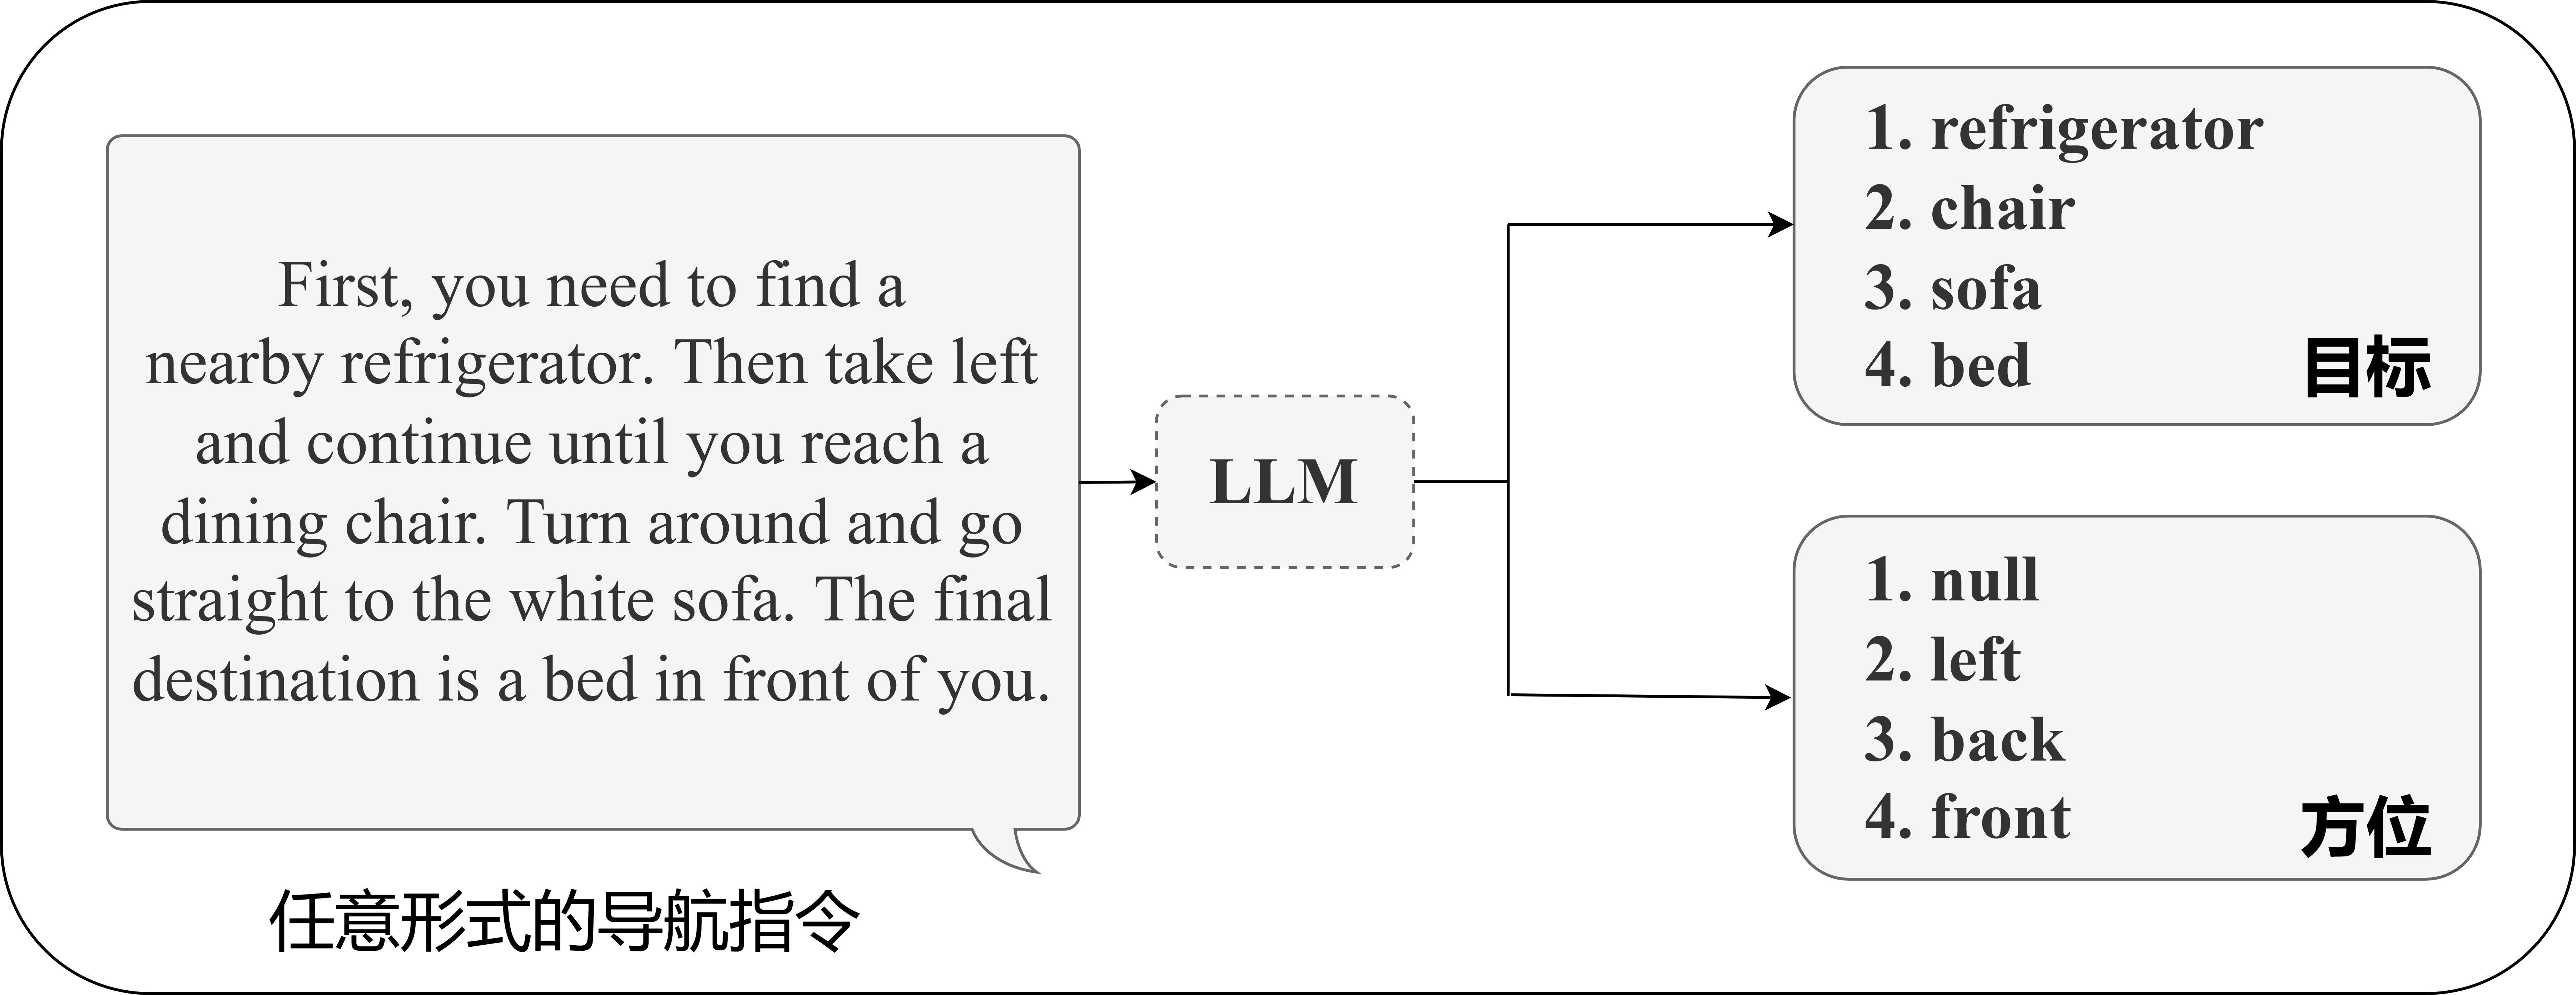
\includegraphics[scale=0.05]{Fig/Extract_orien.png}
    \caption{\label{Extract_orien}指令语义提取模块}
\end{figure}




\section{多模态融合网络模块}
CLIP(Contrastive Language-Image Pre-training)多模态融合网络\cite{radford2021learning}是一种基于对比学习的多模态融合模型,它通过将图像和文本映射到同一个嵌入空间中使匹配的图像-文本对的特征向量尽可能接近,不匹配的图像-文本对的特征向量尽可能远离。这种学习策略使得CLIP在没有特定任务训练数据的情况下依然能够有效地执行分类和搜索任务,使得该模型展现出极高的泛化能力和适应性。因此CLIP依靠其具有的极大灵活性和通用性在众多计算机视觉和自然语言处理任务中展现出优越的性能,同时也在多模态建模领域得到了广泛关注。

在利用视觉语言进行导航的任务中,一个核心挑战是如何高效且准确地将语义目标与环境图像进行匹配,并在此基础上规划出一条符合指令描述的全局导航点序列,以确保导航智能体能够按照预期完成路径规划。InteriorNet\cite{li2018interiornet}是由帝国理工学院和KooLab联合创建的大规模、多传感器、照片级真实感室内场景数据集,该数据集包含约100万个来源于真实的生产制造的家具CAD模型和2200万个室内布局。为了研究CLIP模型在不同光照环境下的表现,我们随机选取了该数据集中的若干图像并通过计算直方图将其划分为4个曝光程度不同的子数据集。这4个子数据集分别对应图像过度欠爆、轻微欠爆、正常曝光、明显过曝的情况。随后使用CLIP模型在这些数据集上进行了图像-文本匹配测试以此评估模型在不同光照条件下匹配的正确率。实验结果如表\ref{Matching_accuracy}所示,这表明在光照条件良好的室内环境下CLIP能够稳定且可靠地完成图像与文本的匹配任务,但当图像出现曝光过度或欠曝的情况时,CLIP的图像-文本匹配正确率却明显下降并表现出较大的不稳定性。这一实验表明尽管CLIP在标准光照条件下能够提供较为理想的匹配效果,但其在室内的复杂光照环境下仍然存在一定的局限性。

\begin{table}[ht]
	\centering
	\caption{模型进行图像文本匹配的正确率} % 表格标题
	\begin{tabular}{ccccc} % 这里定义了列的格式
	\toprule % 上方的横线
	色阶范围 & [0,60] & [61,120] & [121,180] & [181,255]  \\ % 表头行
	\midrule % 中间的横线
	CLIP & 32.43\% & \textbf{99.12\%} & 89.38\% & 37.72\% \\ % 第一行数据
	CLIDP & \textbf{44.95\%} & 98.23\% & \textbf{92.04\%} & \textbf{42.28\%} \\ % 第二行数据
	\bottomrule % 底部的横线
	\end{tabular}
	\label{Matching_accuracy}
\end{table}

为了解决现有视觉语言导航系统在不同光照条件下匹配能力不稳定的问题,本文针对多模态融合网络的特征提取能力进行了改进,引入了一种深度图像编码器以提取环境中的深度信息从而扩展了模型所能捕捉的特征维度。这种改进能够确保模型在曝光过度或欠曝的复杂光照条件下,仍然可以依赖深度特征信息进行准确的图像-文本匹配,而不仅依赖于颜色或纹理等受光照影响较大的视觉特征。基于这一思路,我们提出了一种新的多模态融合框架CLIDP(Contrastive Language-Image-Depth Pre-training),其整体架构如图\ref{CLIPD_framework}所示。
\begin{figure}[htbp]
    \centering
    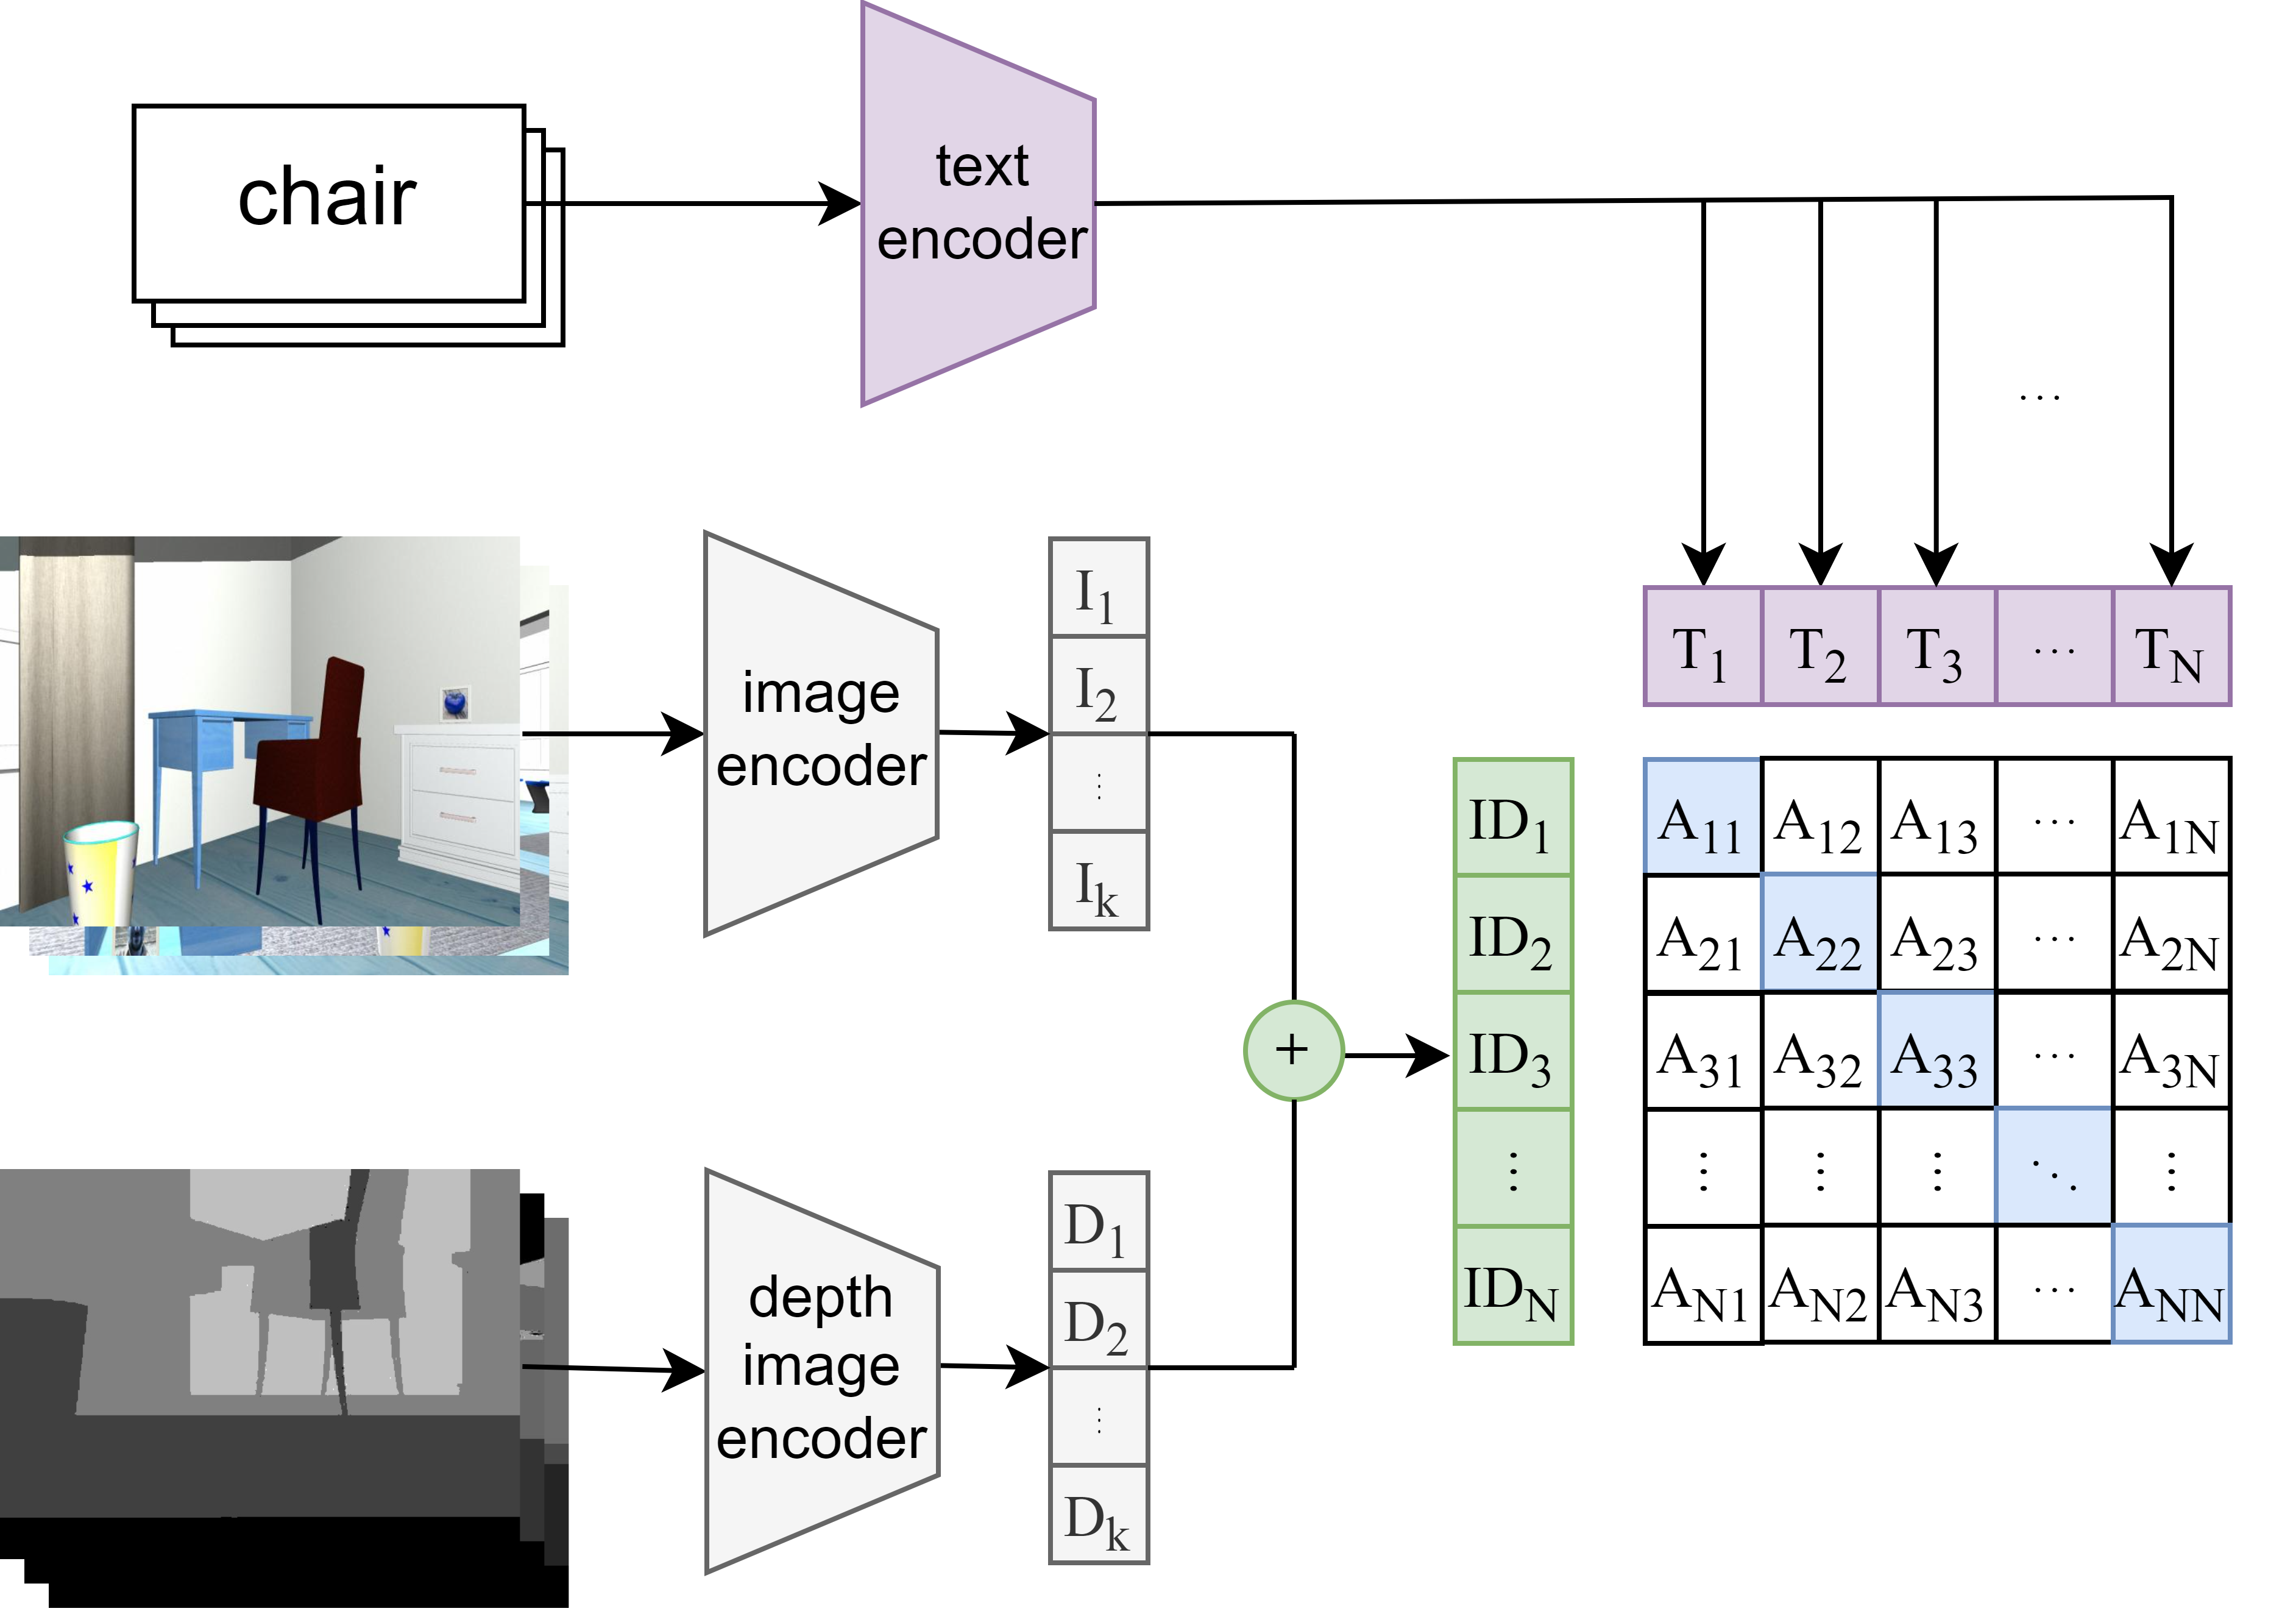
\includegraphics[scale=0.09]{Fig/CLIPD_framework.png}
    \caption{\label{CLIPD_framework}CLIPD多模态融合网络框架}
\end{figure}

CLIDP多模态融合网络在预训练模型ViT-B-32\cite{radford2021learning}的基础上,通过引入的深度信息进行了进一步的优化和重训练,其意在解决的关键任务是在给定的((图像,深度图),文本)数据对中,预测其中存在的所有可能配对的概率。
这一过程通过训练一个图像编码器和一个深度图编码器来分别提取环境的RGB图像和深度特征信息,并将这两个部分的特征拼接,以形成完整的环境特征表示。

首先,图像编码器使用与CLIP类似的ViT(Vision Transformer)结构,如图\ref{viT}所示,图像切分与嵌入(Patch Embedding)操作会将输入的图像划分为固定大小的非重叠小块,并将小块通过线性变换投影到高维特征空间形成Patch嵌入向量,通过将大尺度的图像分解成更小的部分可以获得更细粒度的信息,帮助模型更好地理解图像内容,接着位置编码(Position Embedding)则会给每个独立的Patch叠加一个可学习的正余弦位置编码使模型能够区分不同位置的Patch,提高空间信息建模能力,然后在编码器(Transfomer Encoder)处通过由多层自注意力机制、前馈神经网络和残差连接等组成的Transfomer结构对每个独立的Patch进行特征提取以捕获全局依赖关系,最后,在分类头(Classification Head)通过MLP进行分类,输出最终预测结果。
\begin{figure}[htbp]
    \centering
    \includegraphics[scale=0.067]{Fig/viT.png}
    \caption{\label{viT}Vision Transfomer结构}
\end{figure}

深度图编码器则使用基于深度残差网络(Deep Residual network)的ResNeet架构,通过引入跳跃连接和注意力机制,从而在解决了深层网络中梯度消失的问题的同时,提高模型对深度特征的识别和利用能力。此外,模型还联合训练一个文本编码器,以从文本指令中提取语义特征,并通过最大化数据集中互相匹配的环境特征与文本特征的余弦相似度\eqref{myeq8},确保模型能够准确地学习环境特征和语言文本特征之间的对应关系。除此之外,在训练过程中我们采用反向传播算法不断优化多模态融合网络的参数,使模型在多种环境条件下都能可靠地进行匹配。其核心训练流程的伪代码如图\ref{CLIDP_CODE}所示。


我们在相同的数据集上对CLIDP网络的图像-文本匹配准确率进行了测试,实验结果如表\ref{Matching_accuracy}所示。通过对比分析可以看出CLIDP在光照条件复杂的室内环境中尤其是在曝光过度或欠曝光的情况下表现出了显著的优势,与原始CLIP模型相比其匹配准确率依然保持较高水平。这表明CLIDP通过融合深度信息使多模态网络能够更有效地感知和理解场景结构,从而增强了模型对光照变化的鲁棒性。这一改进能够提升CLIDP在复杂室内环境下的图像-文本匹配精度,使其在现实应用中具有更强的适应能力。多模态融合网络CLIDP为后续的导航点规划算法提供可靠的目标-图像匹配信息。
\begin{equation}
    \cos \left( \theta  \right) = \frac{{A \times B}}{{\left\| A \right\|\left\| B \right\|}} = \frac{{\sum\limits_{i = 1}^n {{{\rm A}_i}{{\rm B}_i}} }}{{\sqrt {\sum\limits_{i = 1}^n {{{\rm A}_i}^2} } \sqrt {\sum\limits_{i = 1}^n {{{\rm B}_i}^2} } }}
        \label{myeq8}
    \end{equation}

\begin{figure}[H]
    \begin{lstlisting} 
    # image_encoder	        - Vision transformer
    # depth_image_encoder	- Vision transformer
    # text_encoder	        - Text transformer
    # I[n, h, w, c]	        - 预处理图像集
    # D[n, h, w, c]	        - 预处理深度图集
    # T[n, l]	            - 预处理文本集
    #W_i[d_i, d_e]	        - 图像学习权重
    #W_d[d_d, d_e]	        - 深度图学习权重
    #W_t[d_t, 2 * d_e]	    - 文本学习权重
    # 提取每个模态的特征
    I_f = image_encoder(I)	        # [n, d_i]
    D_f = depth_image_encoder(D)	# [n, d_d]
    T_f = text_encoder(D)	        # [n, d_t]
    # 多模态嵌入
    I_e = l2_normalize(np.dot(I_f, W_i), axis = 1)	#[n, d_e]
    D_e = l2_normalize(np.dot(D_f, W_d), axis = 1)	#[n, d_e]
    T_e = l2_normalize(np.dot(T_f, W_t), axis = 1)	#[n, 2*d_e]
    # 环境特征
    ID_e = np.concatenate(I_e, D_e, axis = 1)
    # 余弦相似度
    logits = np.dot(ID_e, T_e.T)
    # 构造损失函数
    labels = np.arange(n)
    loss_id = cross_entropy_loss(logits, labels, axis = 0)
    loss_t = cross_entropy_loss(logits, labels, axis = 1)
    loss = (loss_id + loss_t) / 2
    \end{lstlisting}
    \caption{CLIDP实现的核心伪代码}
    \label{CLIDP_CODE}
    \end{figure}
    



\section{方位优化算法}
传统的视觉语言导航方法主要依赖于从图像中提取的目标特征和环境特征进行推理导航,但在包含多个相同物体的复杂室内环境之中,图像中的目标特征和环境特征会交织在一起,并且会忽略目标与其他物体之间的空间位置关系,导致视觉语言导航的准确率下降。此外,第一人称视觉观察中的所有物体视觉信息都会被同时处理,这要求代理需要在环境中所有可能的物体中进行判断,可能会浪费大量的时间去处理与目标关联度较小的物体,而这种情况在目标物体不显眼、环境物体过多的环境中尤为突出,这增加了后续模型计算推理的复杂性,同时也降低了导航的效率,并且可能导致计算效率低下。

在室内环境进行视觉语言导航的实验中,当环境的多个不同位置都包含相似或相同的物品时,智能体难以仅仅依赖多模态融合网络和Dijkstra算法根据自然语言指令准确执行导航任务。为了解决这一问题本文引入了一种方位优化算法,它通过分析自然语言指令中包含的方位语义来有效地筛选出冗余的导航点进而改善导航路径的准确性和效率。具体而言,通过语言模型可以从各种形式的自然语言指令中提取出null、front、back、left和right这五种常见的方位指代。这些方位指代帮助代理在进行导航规划时不需要考虑环境中所存在的所有导航点,而是专注于与目标物体相关的区域和物体从而更高效地筛选出有用的信息,同时也能达到减少不必要的计算的目的,避免了在视觉上和空间上不相关的物体对目标识别的干扰。除此之外,这种方位优化方法还能辅助代理确定目标位置与当前机器人位姿之间的相对方位,让代理在环境复杂、物体众多的情况下也能专注于目标物体所在的特定区域而不会受到无关物体的干扰,剔除那些不在指定方位上的冗余导航点从而使代理可以更快、更准确地到达目标,这也增强了导航系统的整体性能。方位优化过程能够大幅提升全局路径规划中生成导航点序列的准确度,使得导航路线更加贴合指令的要求。在第五章中我们通过仿真实验和消融实验验证了该方位优化算法在室内环境下进行视觉语言导航的有效性。

在ROS(Robot Operating System)系统中,每个导航点的坐标都是基于地图坐标系(map)来定义的。为了实现精确的路径规划和导航,必须通过坐标变换将基于地图坐标系下的导航点坐标转换为机器人当前位姿坐标系下的坐标,如图\ref{axis_transform}所示。这一数学转换可以通过式\eqref{myeq9}进行。
\begin{figure}[htbp]
    \centering
    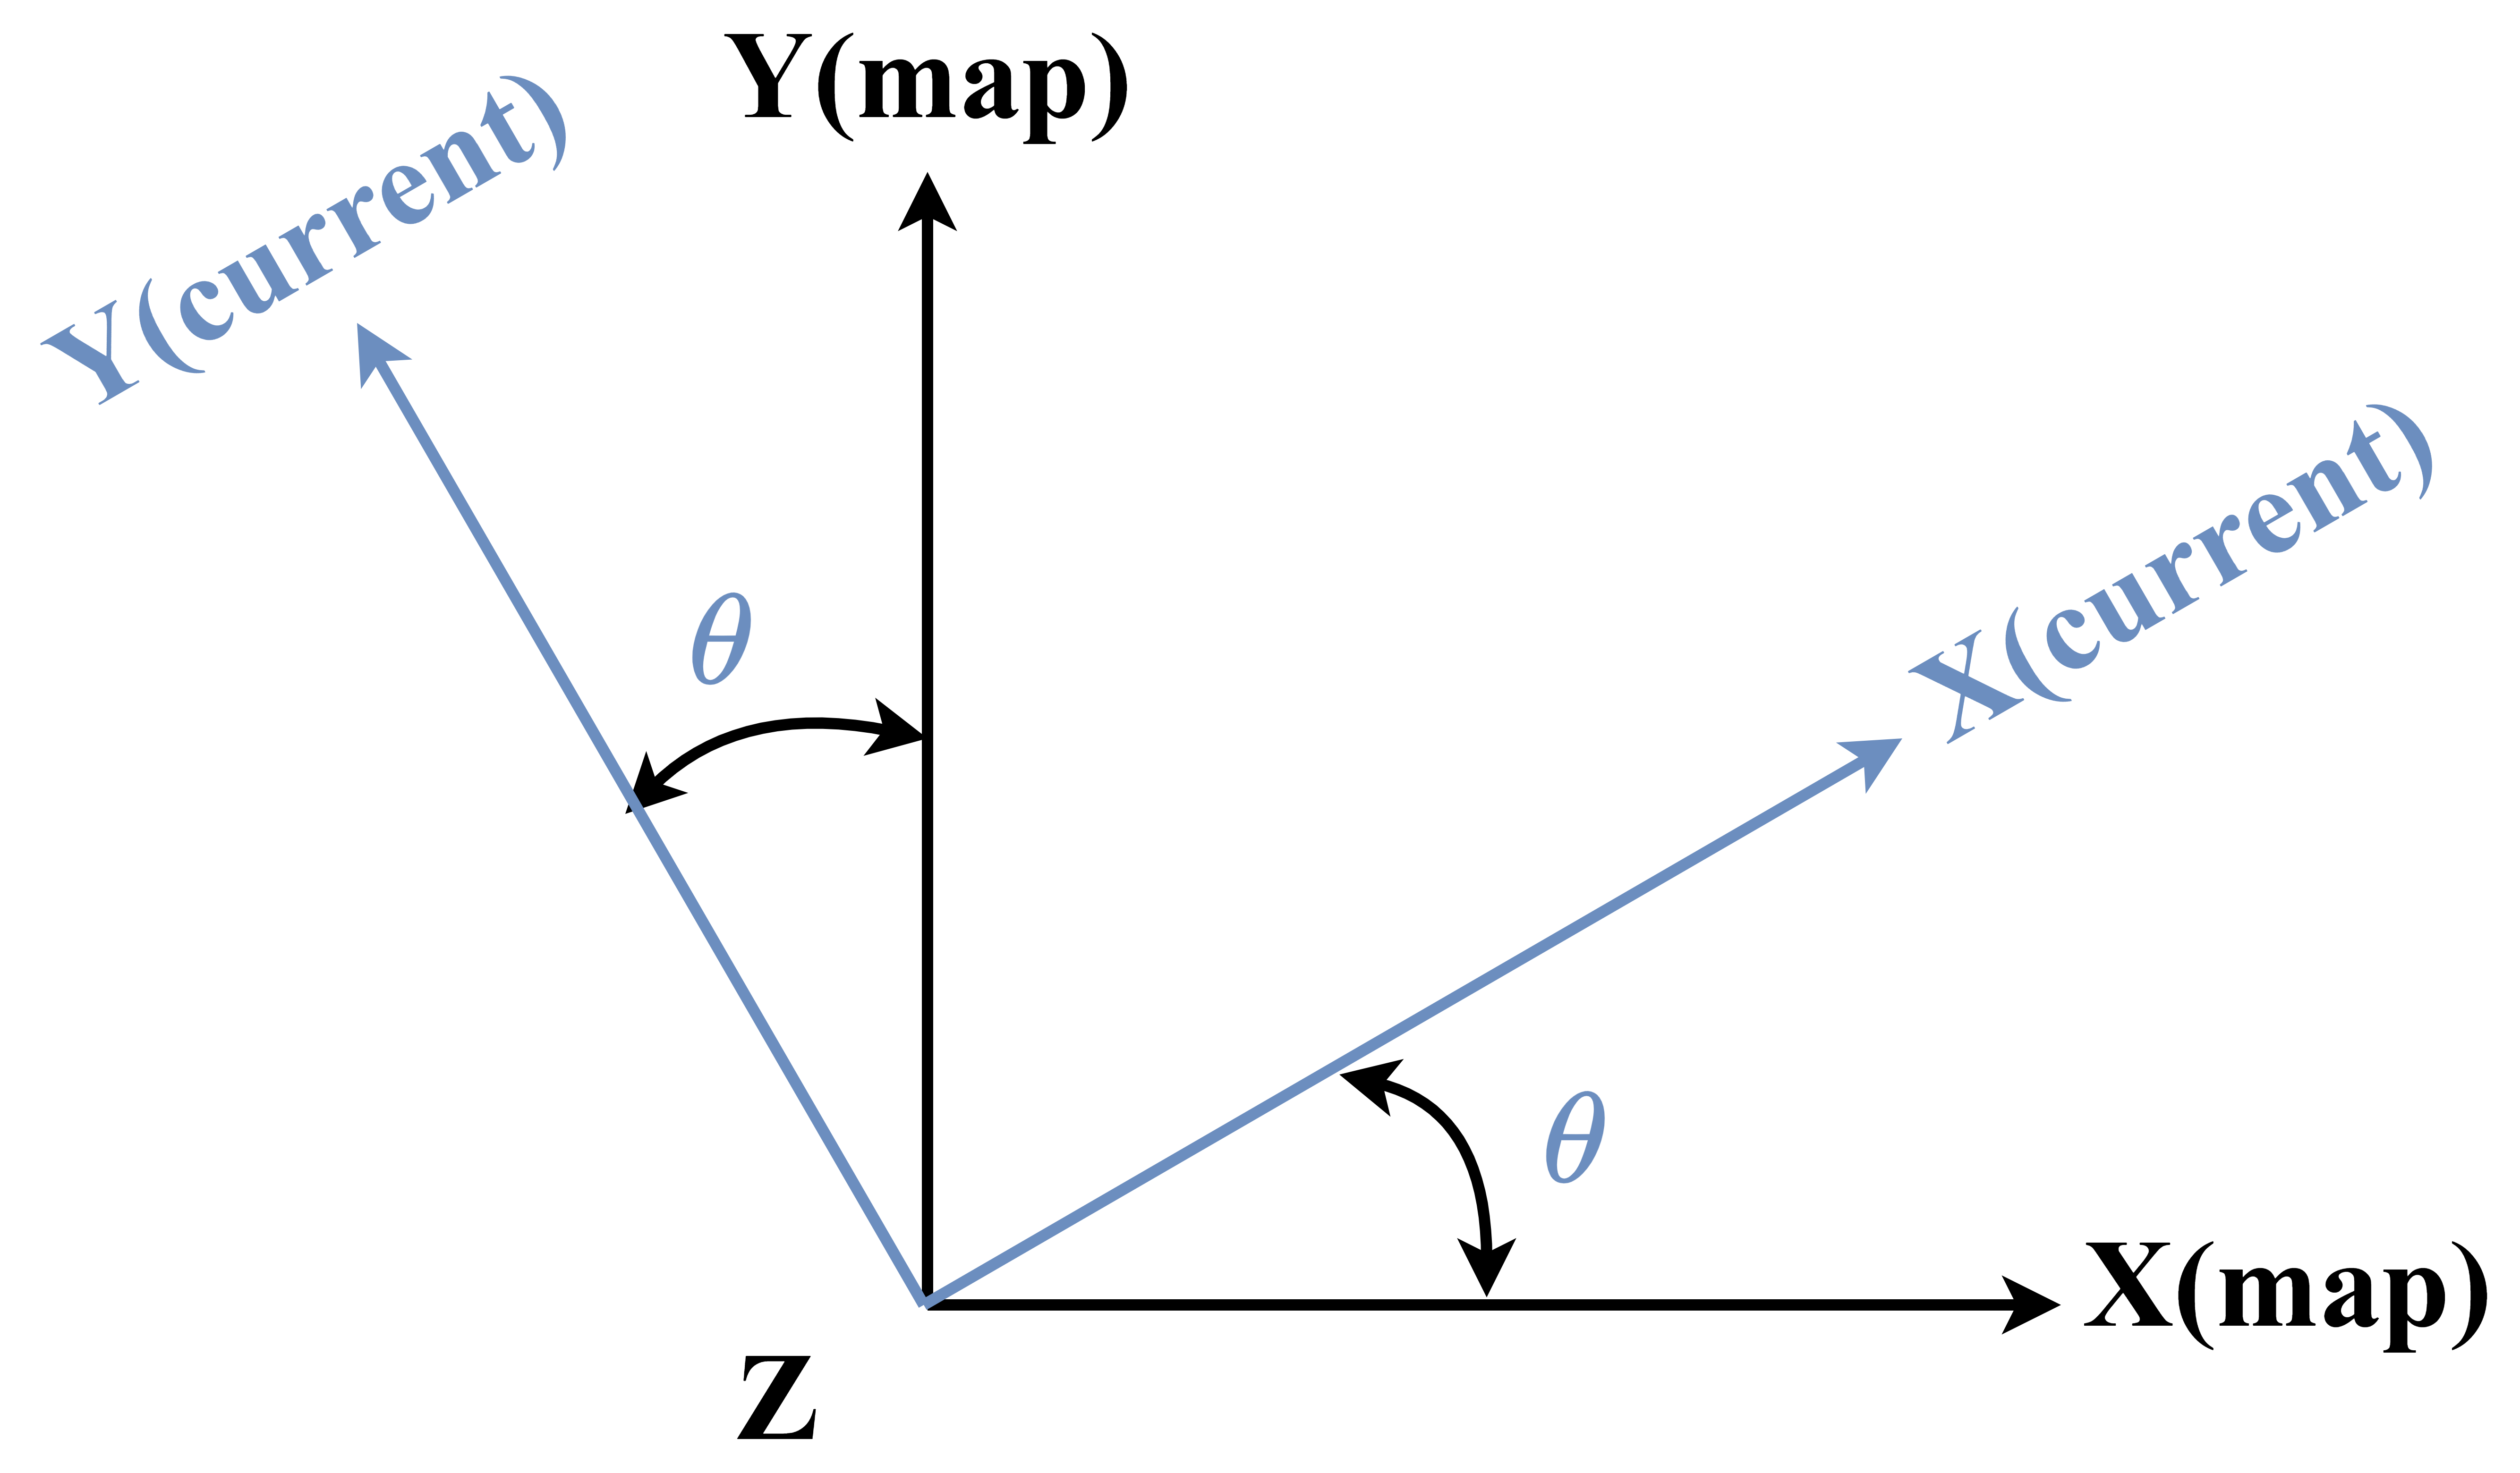
\includegraphics[scale=0.06]{Fig/axis_transform.png}
    \caption{\label{axis_transform}地图与实时位姿坐标变换}
\end{figure}
\begin{equation}
{P_B}^\prime  = \left( {\begin{array}{*{20}{c}}
{\cos \theta }&{\sin \theta }\\
{ - \sin \theta }&{\cos \theta }
\end{array}} \right)\left( {{P_B} - {P_A}} \right)
\label{myeq9}
\end{equation}
其中${{P_A}}$表示机器人在地图坐标系中的位置,${{P_B}}$表示某个导航点在地图坐标系中的位置,${P_B}^\prime$表示导航点在机器人坐标系下的相对位置,而$\theta$则表示机器人在地图坐标系中的偏航角,它代表了机器人当前位置相对于地图坐标系的旋转角度。通过计算这一角度,可以将环境中的所有导航点坐标转换为机器人坐标系中的坐标,从而确保全局路径规划中的导航点坐标是准确的。

然而,偏航角$\theta$本身无法直接测量或获得,它必须通过旋转矩阵进行求取。在ROS的Navigation框架中,可以使用tf库中的TransformListener来监听机器人在地图坐标系下的位姿信息。位姿信息是通过四元数$q = (x, y, z, w)$来表示的,其中$(x, y, z)$表示机器人的位置,而$w$则表示旋转参数。通过监听对应话题获取这一四元组后,便可以将四元组转换成式\ref{myeq10}表示的旋转矩阵$R$
\begin{equation}
	R = \left[ {\begin{array}{*{20}{c}}
		{1 - 2{y^2} - 2{z^2}}&{2\left( {xy - zw} \right)}&{2\left( {xz + yw} \right)}\\
		{2\left( {xy + zw} \right)}&{1 - 2{x^2} - 2{z^2}}&{2\left( {yz - xw} \right)}\\
		{2\left( {xz - yw} \right)}&{2\left( {yz + xw} \right)}&{1 - 2{x^2} - 2{y^2}}
		\end{array}} \right]
	\label{myeq10}
\end{equation}

除此之外,机器人当前的位姿的欧拉角是在地图坐标系下,分别通过绕X轴旋转$\gamma$角、绕Y轴旋转$\beta$角以及绕Z轴旋转$\alpha$角获得的。这些角度的组合构成了机器人在地图坐标系下的完整姿态。式\ref{myeq11}给出了旋转矩阵的计算方式,通过这个旋转矩阵可以有效地表示机器人在地图坐标系中的朝向。
\begin{equation}
	{R_{XYZ}}\left( {\gamma ,\beta ,\alpha } \right) = \left[ {\begin{array}{*{20}{c}}
		{c\alpha  \cdot c\beta }&{c\alpha  \cdot s\beta  \cdot s\gamma  - s\alpha  \cdot c\gamma }&{c\alpha  \cdot s\beta  \cdot c\gamma  + s\alpha  \cdot s\gamma }\\
		{s\alpha  \cdot c\beta }&{s\alpha  \cdot s\beta  \cdot s\gamma  + c\alpha  \cdot c\gamma }&{s\alpha  \cdot s\beta  \cdot c\gamma  - c\alpha  \cdot s\gamma }\\
		{ - s\beta }&{c\beta  \cdot s\gamma }&{c\beta  \cdot c\gamma }
		\end{array}} \right]
	\label{myeq11}
\end{equation}
式中:${c\alpha }$表示$\cos \alpha $,${s\alpha }$表示$\sin \alpha $

通过联立式\ref{myeq10}和\ref{myeq10}可以通过四元组来表示出欧拉角$\alpha $、$\beta $和$\gamma $如式\ref{myeq12}
\begin{equation}
	\begin{array}{c}
\beta  = {\rm{Atan2}}\left( { - {r_{31}},\sqrt {r_{11}^2 + r_{21}^2} } \right)\\
\alpha  = {\rm{Atan2}}\left( {\frac{{{r_{21}}}}{{c\beta }},\frac{{{r_{11}}}}{{c\beta }}} \right)\\
\gamma  = {\rm{Atan2}}\left( {\frac{{{r_{32}}}}{{c\beta }},\frac{{{r_{33}}}}{{c\beta }}} \right)
\end{array}
\label{myeq12}
\end{equation}
其中${{r_{ij}}}$表示旋转矩阵中第i行第j列元素,${\rm{Atan2}}\left( {x,y} \right)$表示$x/y$的反正切值。

式\ref{myeq12}计算得到的角度$\alpha$,即为机器人当前位姿在地图坐标系中的偏航角$\theta$,将其代回式\ref{myeq9}进行坐标转换,可以计算出各个地图坐标系线下的导航点在机器人坐标系下的精确坐标。通过与语言模型解析的方位指令进行对比,系统能够筛选出哪些导航点位于指令所指定的方位范围内,从而剔除那些不符合指令要求的冗余导航点,为机器人提供精确的路径点序列。这一优化过程显著提升了机器人在执行视觉语言导航任务时的准确性和效率。



\section{导航点规划算法}
在拥有环境拓扑图的导航点选择任务中通常会使用Dijkstra算法进行决策,根据最短距离的贪心思路帮助移动机器人进行导航点的选择,以期更快地找到目标。然而这种方法无法将导航目标与环境物体和物体之间的位置关系结合起来,且这种导航方法大多使用于静态的导航环境之中,对于可能会因为物体的摆放而改变可导航路径的复杂环境会使得原本的拓扑图失效,降低代理导航正确率和导航效率。基于这一思路,我们给全局路径规划任务进行建模,设计了一种全新的导航点规划算法。

全局路径规划可以描述为在遵循自然语言指令中给出的目标的情况下最大化导航成功的概率。具体来说,室内导航环境可以由一系列的房间$E = {e_1},{e_2}, \ldots ,{e_k}$共同组成,环境中存在由一系列导航点$V = {v_1},{v_2}, \ldots ,{v_n}$组成的拓扑图$G$,图中的节点代表了环境中的枢纽,边的权值则代表一个节点导航到另一个节点的路径代价。一次导航任务$\tau  \in D$由导航环境、拓扑图、初始位姿$S$和导航指令$I$确定,因此我们将每次导航任务表示成$\tau  = \left( {E,G,S,I} \right)$。在先前的小节中我们通过指令语义提取模块对导航指令$I$进行解析,提取出导航指令中的目标序列$\bar l = {l_1},{l_2}, \ldots ,{l_n}$,导航点规划算法就是要找到一个导航点序列$\bar v = {v_1},{v_2}, \ldots ,{v_n}$,使得该序列能够最大化目标与导航点之间的匹配程度,并尽可能提高导航成功率,如式\ref{myeq13}。
\begin{equation}
	P\left( {{v_i}|{l_i}} \right)P\left( {{c_{\bar v}} = 1|\bar v} \right) = \mathop {\max }\limits_{1 \le {t_i} \le  \cdots  \le {t_n} \le n} \prod\limits_{1 \le i \le n} {p\left( {{v_{{t_i}}}|{l_i}} \right) \cdot \prod\limits_{1 \le j \le n} {{\mu ^{Dis\left( {{v_j},{v_{j + 1}}} \right)}}} } 
	\label{myeq13}
\end{equation}
其中$P\left( {{c_{\bar v}} = 1|\bar v} \right)$表示根据导航点序列$\bar v$能够完成导航的概率,$P\left( {{v_i}|{l_i}} \right)$表示导航节点${v_i}$与给定的一个目标${l_i}$相匹配的概率,该概率通过多模态融合网络进行预测输出,$\mu  \in \left( {0,1} \right)$,${{\mu ^{Dis\left( {{v_j},{v_{j + 1}}} \right)}}}$代表从导航节点${{v_{j}}}$导航到${{v_{j + 1}}}$的距离代价,即随着拓扑图中所存在的任意两个导航点${v_j}$与${v_{j + 1}}$距离的增大,他们成为自然语言指令所指示的导航任务中相邻导航点的概率越小。

为了求得式\ref{myeq13}一个最优的解${\bar v}$,我们对其进行求导,得到一个对于序列$\bar t = {t_1},{t_2}, \ldots ,{t_n}$单调递增的函数:
\begin{equation}
	R\left( {\bar v,\bar t} \right) = \sum\limits_{i = 1}^n {{\rm{CLIDP}}\left( {{v_{{t_i}}},{l_i}} \right) + \log \left( \mu  \right) \cdot \sum\limits_{j =  = 1}^{T - 1} {{\rm{Dis}}\left( {{v_j},{v_{j + 1}}} \right)} } 
	\label{myeq14}
\end{equation}
当且仅当$\left( {\bar v,\bar t} \right)$最大化式\ref{myeq14}时,可以同时使得序列${\bar v}$最大化式\ref{myeq13}

为了求得最大化式\ref{myeq13}的解$\left( {\bar v,\bar t} \right)$,可以通过构造一个辅助函数,再利用动态规划的方法得到$R$的全局最优解。综上所述,对于$\forall i \in \left\{ {0,1, \ldots ,n} \right\}$和$\forall v \in V$,定义一个辅助函数$Q\left( {i,v} \right)$,表示以$v$结尾的所有导航点序列与目标点序列$\left( {{l_1},{l_2}, \ldots ,{l_n}} \right)$匹配的的最大值:
\begin{equation}
	Q\left( {i,v} \right) = \mathop {\max }\limits_{\scriptstyle\bar v = \left( {{v_1},{v_2}, \ldots ,{v_j}} \right),{v_j} = v\atop
\scriptstyle\bar t = \left( {{t_1},{t_2}, \ldots ,{t_i}} \right)} R\left( {\bar v,\bar t} \right)
	\label{myeq15}
\end{equation}

我们通过算法\ref{algorithm2}描述了结合环境拓扑图、多模态融合网络的导航点规划算法的具体过程。从起始位姿开始,通过动态规划的方式,最大化目标匹配度和最小化路径代价,以获得全局路径规划输出的导航点序列。
\begin{algorithm}[!h]
    \caption{导航点规划算法}
    \label{algorithm2}
    \renewcommand{\algorithmicrequire}{\textbf{Input:}}
    \renewcommand{\algorithmicensure}{\textbf{Output:}}
    \renewcommand{\algorithmiccomment}[1]{\hfill $\triangleright$ #1}
    \begin{algorithmic}[1]
        \REQUIRE 目标序列$\bar l = {l_1},{l_2}, \ldots ,{l_n}$,拓扑图$G$,起始位姿$S$和指令$I$  %%input
        \ENSURE 导航点序列${\rm{Path}} = \left[ {\bar v = {v_1},{v_2}, \ldots ,{v_n}} \right]$   %%output
        \STATE  对$\forall i \in 1,2, \ldots ,n$和$\forall v \in V$初始化$Q\left( {i,v} \right) =  - \infty $
        \STATE  初始化$Q\left( {0,v} \right)$
        \FOR{$i \in 1,2, \ldots ,n$}
            \STATE  对$\forall v \in V$,通过递推公式求解$Q\left( {i,v} \right)$
            \STATE  Path中添加导航点$\left( {{\rm{argmax}}\left( {Q\left( {i, * } \right)} \right)} \right)$
			\STATE  $S = {\rm{argmax}}\left( {Q\left( {i, * } \right)} \right)$
        \ENDFOR
    \end{algorithmic}
\end{algorithm}

在上述的导航点规划算法中,首先输入通过语言模型提取的目标序列和环境拓扑图,设置导航起始点$S$,初始化$Q\left( {0,v} \right)$为导航起始点$S$到各个导航点$v$的最短路径长度,当$i \ge 1$时,我们通过动态规划递推公式计算每一时刻的$Q(i, v)$值:
\begin{equation}
Q\left( {i,v} \right) = \max \left( {Q\left( {i - 1,v} \right) + {\rm{CLIDP}}\left( {v,{l_i}} \right),\mathop {\max }\limits_{\omega  \in {\rm{neighbors}}\left( v \right)} \lambda  \cdot Q\left( {i,\omega } \right) + \mu  \cdot Dis\left( {v,\omega } \right)} \right)
	\label{myeq16}
\end{equation}
其中,${{\rm{neighbors}}\left( v \right)}$表示拓扑图中节点$v$的邻接点,$\lambda  \in \left( {0,1} \right)$表示缩放参数,目的是减少先前的导航点选择对后续决策的影响。在每一次的递推过程中,我们采用贪心策略选取能够使得$Q\left( {i,v} \right)$取得最大值、且经过方位优化筛选后的节点作为当前目标所对应的导航点,并将其设为下一递推过程的起点,直到遍历完目标序列,得到全局路径规划的导航点序列$\bar v = {v_1},{v_2}, \ldots ,{v_n}$。




\section{本章小结}
本章主要内容是目标物体导航过程中涉及到的一些常用的网络在导航过程中的作用以及这些网络的算法原理和操作流程,主要介绍了指令语义提取模块、多模态融合网络模块、方位优化算法和导航点规划算法。




